\documentclass[11 pt]{article}
\usepackage{structure}


\title{LMECA2300 - Advanced numerical methods - Assignment 4}
\author{
    DEGROOFF\\ Vincent\\ 09341800
    \and
    HENNEFFE\\ Christophe\\ 14831800
    \and
    MOUSAVI BAYGI\\ Seyedeh Toktam\\ 08172101
}
\date{Friday 13 May 2022}

\begin{document}

\maketitle

\section{Analytical and numerical solution comparison}

We consider a test case without mean flow, and with a speed of sound $c=1$ m/s. The initial pressure condition has a centered Gaussian distribution:
\begin{equation*}
    p(x,y, 0) = e^{-20(x^2+y^2)}
\end{equation*}

The initial conditions $u(x,y,t=0)$ and $v(x,y, t=0)$ are both zero everywhere.

Using the formula from \cite{TAM1993262}, the analytical solution is then given by
\begin{equation*}
    p(x,y,t) = \frac{1}{40} \int_0^{\infty}e^{-\frac{\xi^2}{80}}\cos (\xi t) J_0(\xi \eta) d\xi
\end{equation*}

where $J_0$ is the Bessel function of the first kind, with order $0$.

\begin{figure}[H]
    \centering
    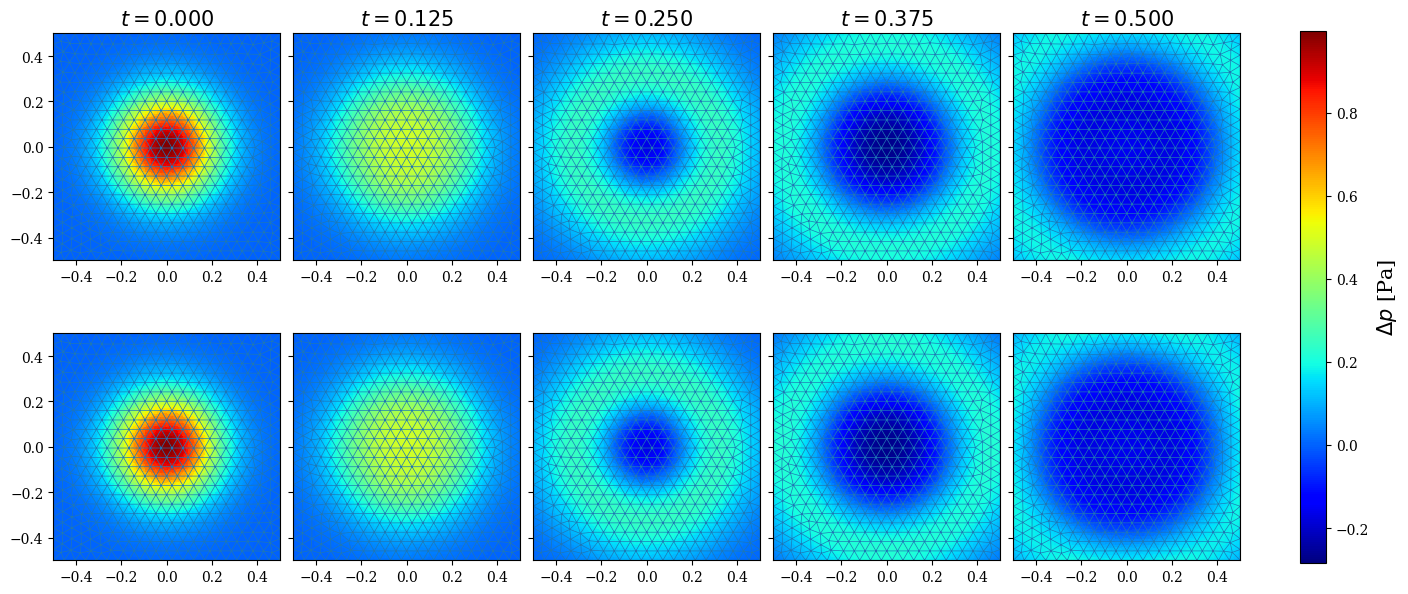
\includegraphics[width=\textwidth]{../figures/comparison.png}
    \caption{Comparison between the analytical (above) and the numerical (below) solutions. The $x$ and $y$ axes are both expressed in meters, and the time units are seconds.}
    \label{fig:comparison}
\end{figure}

The result of the implementation is really close to the solution predicted by the theory. We also observe that the simplified non-reflective boundary condition works really well in this test case. For the record, we implemented the true Riemann solver for the numerical flux.

\section{Slip wall condition}
In this simulation, we implemented a slip wall condition for the lateral walls of a channel. The initial condition is still a Gaussian, centered this time at $(175, 125)$. We then solved the Euler equations with 3 different mean flows: subsonic $M=0.5$, transonic $M=1.$ and supersonic $M=1.5$.
\begin{figure}[H]
    \centering
    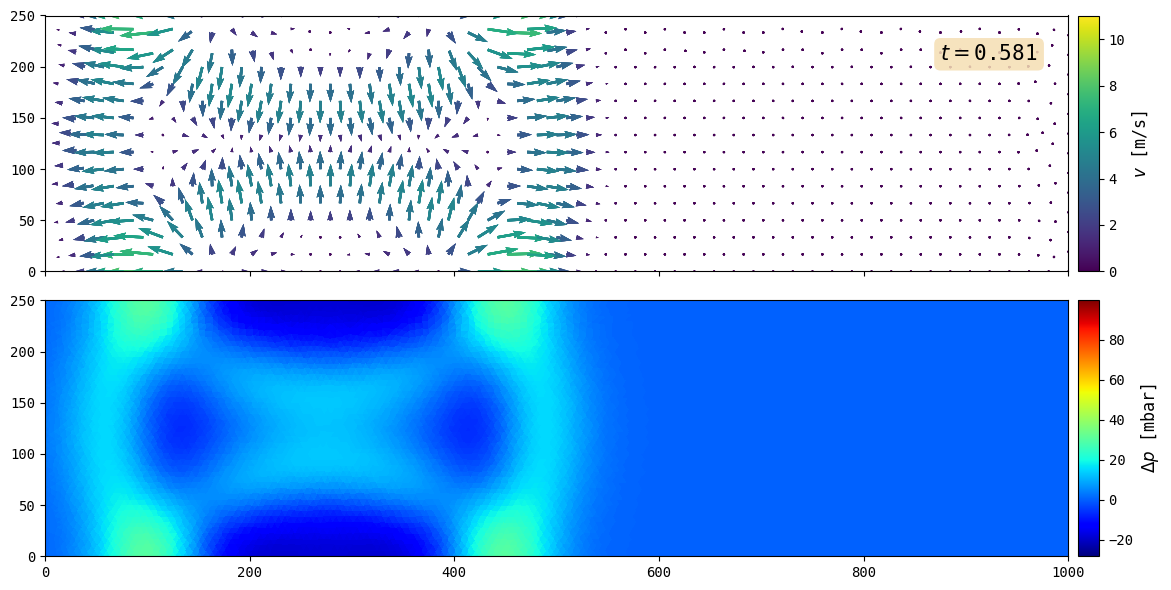
\includegraphics[width=\textwidth]{../figures/simu_1.png}
    \caption{Simulation in a channel at $M=0.5$.}
    \label{fig:channel_subsonic}
\end{figure}

The results in the other cases are quite similar: they are simply being shifted to the right since the mean flow $u_0$ is increased. Therefore, we will not show more images of these simulations. However, we made videos that are available in the directory \texttt{Animations} that show the differences between the 3 cases.

\section{Doppler effect with a periodic source}
The source $f(x,y,t)$ is modeled as a Gaussian peak, repeated periodically every $0.25$ second. The period is $25$ times longer than the duration of the peak, which is thus $\Delta t = 0.01$ second.

\begin{align*}
    f(x,y,t) &= \epsilon_1 \exp\big[-\alpha_1 (x_c^2+y_c^2)\big] g(t)\\
    g(t) &= \exp\left[-\frac{t^2}{2 \left(\frac{0.025}{25}\right)^2}\right]
\end{align*}

where $\epsilon_1=10^4$, $\alpha_1=5$, $x_c=x-250$, $y_c=y-125$, $g(t)$ is repeated periodically, and the channel keeps the same dimensions $L=1000$ m and $H=250$ m.

\begin{figure}[H]
    \centering
    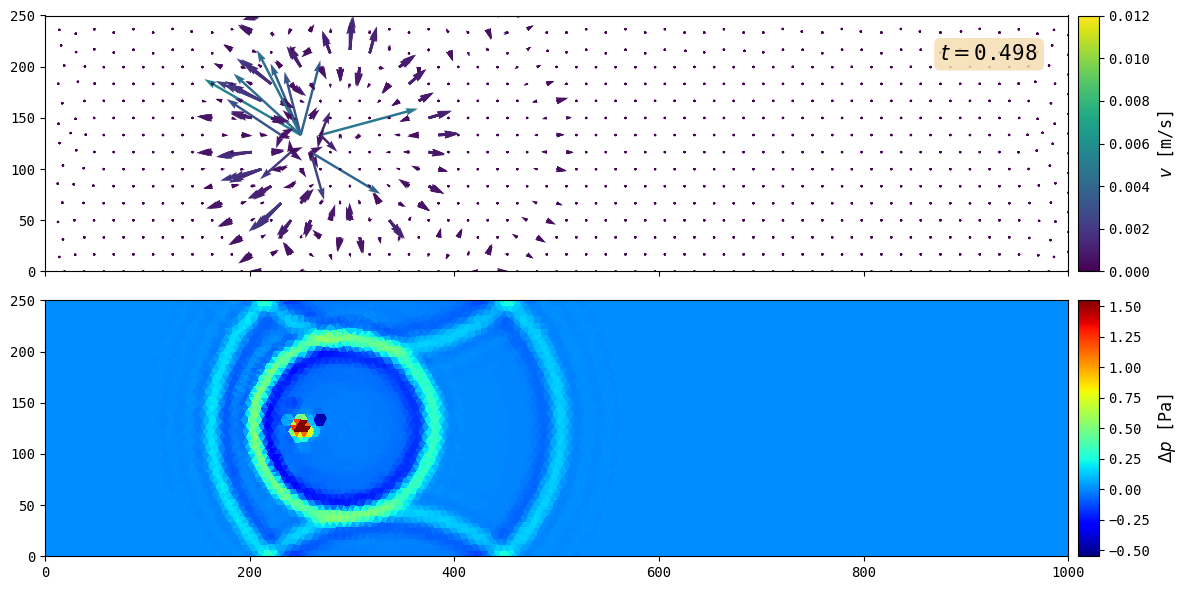
\includegraphics[width=\textwidth]{../figures/doppler_1.png}
    \caption{Periodic source in a channel at $M=0.5$.}
    \label{fig:doppler_transonic}
\end{figure}

In figure \ref{fig:doppler_transonic}, we can clearly see how the wave is distorted due to the mean flow. The wave traveling to the left moves at a speed $c-u_0=170$ m/s, while the wave traveling to the right moves at a speed $c+u_0=510$ m/s.

Once again, videos of the Doppler effect are available in the directory \texttt{Animations}. There are 3 videos: subsonic $M=0.5$ as in figure \ref{fig:doppler_transonic}, transonic $M=1.$ and supersonic $M=1.5$. In the transonic case, we can observe a vertical shock-wave created at the location of the source. In the supersonic case, as expected, we can observe that the pattern of the waves forms a cone.


\nocite{*}
\printbibliography

\end{document}
